\chapter{Some Notes on HOPS}
\label{chap:hops_notes}
\section{Normalized HOPS}%
\label{sec:norm}
In this short note we introduce a \emph{stable} norm preserving term
into the HOPS equations.

We introduce the full HOPS vector \(Ψ = \qty(ψ, φ)\) which can be
decomposed into the zeroth hierarchy order state \(ψ\) and the
non-zero order states \(φ\).

The HOPS equations can then be written in an abstract manner as
\begin{equation}
  \label{eq:HOPS}
  \begin{aligned}
    \dot{ψ} &= F(ψ, φ), & \dot{φ} &= G(ψ, φ),
  \end{aligned}
\end{equation}
where \(c\cdot F(ψ, φ) = F(c\cdot ψ, c\cdot φ)\) and
\(c\cdot G(ψ, φ) = G(c\cdot ψ, c\cdot φ)\) for \(c\in\CC\)


The goal is to transform \(ψ \rightarrow \tilde{ψ}\) so that
\begin{equation}
  \label{eq:goal}
  \norm{\tilde{ψ}} = 1
\end{equation}
in a numerically stable manner.

Introducing the definitions \(\tilde{ψ} = \eu^{f(t)}ψ\) and
\(\tilde{φ} = \eu^{f(t)}φ\) with an
arbitrary\(f\colon \RR \rightarrow \CC\) we can begin to calculate
\begin{equation}
  \label{eq:normdgl}
  ∂_t\norm{\tilde{ψ}}^2 = \tilde{ψ}^† \qty(\dot{f}\tilde{ψ} +
  F(\tilde{ψ}, \tilde{φ})) + \cc = \dot{f} \abs{\tilde{ψ}}^2 +
  \tilde{ψ}^†F(\tilde{ψ}, \tilde{φ}) + \cc.
\end{equation}

We would now like to obtain \(∂_t\norm{\tilde{ψ}}^2 = 0\) as well as
\(\dot{f} > 0\) for \(\norm{\tilde{ψ}} < 1\), \(\dot{f} < 0\) for
\(\norm{\tilde{ψ}} > 1\) and \(\dot{f} = 0\) for
\(\norm{\tilde{ψ}}=1\), so that \(\norm{\tilde{ψ}} = 1\) becomes a
stable fix-point.

Observing \cref{eq:normdgl}, we conclude that our goals can be
achieved by demanding
\begin{equation}
  \label{eq:fdgl}
  \dot{f} = \frac{\tilde{ψ}^†F(\tilde{ψ},
    \tilde{φ})}{\norm{\tilde{ψ}}^2} + g\qty(\norm{ψ}^2)
\end{equation}
with \(g(0)=0\).

The first summand on its own would lead to norm conservation, \(∂_t\norm{\tilde{ψ}}^2 =
0\). The latter of our goals may be achieved by
choosing \(g(x) = \qty(1-x)\).

These choices lead to an altered HOPS equation
\begin{equation}
  \label{eq:normedhops}
  \dot{\tilde{Ψ}} = \qty[\frac{\tilde{ψ}^†F(\tilde{ψ},
    \tilde{φ})}{\norm{\tilde{ψ}}^2}+\qty(1-\norm{\tilde{ψ}}^2)]\mqty(\tilde{ψ}\\
  \tilde{φ}) + \mqty(F(\tilde{ψ},\tilde{φ}) \\ G(\tilde{ψ},\tilde{φ})).
\end{equation}

\section{Multiple Baths}
\label{sec:hops_multibath}

We generalize the NMQSD and HOPS to \(N\) baths for Hamiltonians of
the form~\cref{eq:multimodel}.


\subsection{NMQSD}
\label{sec:nmqsd}

Following the usual derivation of the NMQSD \cite{Diosi1998Mar}, we
switch to an interaction picture with respect to the \(H_\bath\)
leading to
\begin{equation}
  \label{eq:multimodelint}
  H(t) = H_\sys + ∑_{n=1}^N \qty[L_n^†B_n(t) + \hc],
\end{equation}
with \(B_n=∑_{λ} g_λ\nth a_λ\nth\eu^{-\iu ω_λ\nth t}\).

We will discuss the zero temperature case. The finite temperature
methods generalize straight forwardly to multiple baths.  Projecting
on a Bargmann (unnormalized) coherent state basis
\(\qty{\ket{\vb{z}^{(1)},\vb{z}^{(2)},\ldots}=
  \ket{\underline{\vb{z}}}}\) of the baths
\begin{equation}
  \label{eq:projected}
  \ket{ψ(t)} = ∫∏_{n=1}^N{\qty(\frac{\dd{\vb{z}\nth}}{π^{N_n}}\eu^{-\abs{\vb{z}}^2})}\ket{ψ(t,\underline{\vb{z}}^\ast)}\ket{\underline{\vb{z}}},
\end{equation}
where \(N_n\) are the number of oscillators in each bath.


We define
\begin{equation}
  \label{eq:processes}
  η^\ast_n(t) = {\qty(\vb{η}^\ast_t)}_n= -\iu ∑_λg_λ^{(n),\ast} z_λ^{(n),\ast}\eu^{\iu ω_λ\nth t}
\end{equation}
and using
\(\pdv{z_λ^{(n),\ast}}=∫\dd{s}\pdv{η^\ast_n(s)}{z_λ^{(n),\ast}}\fdv{η^\ast_n(s)}\)
we arrive at
\begin{equation}
  \label{eq:multinmqsd}
  ∂_tψ_t(\vb{η}^\ast_t) = -\iu H ψ_t(\vb{η}^\ast_t) +
  \vb{L}\cdot\vb{η}^\ast_tψ_t(\vb{η}^\ast_t) - ∑_{n=1}^N L_n^†∫_0^t\dd{s}α_n(t-s)\fdv{ψ_t(\vb{η}^\ast_t)}{η^\ast_n(s)},
\end{equation}
where \(α_n(t-s)= {\qty(\vb{α}(t-s))}_n=∑_λ\abs{g_λ\nth}^2\eu^{-\iu ω_λ\nth(t-s)}\) are the
zero temperature bath correlation functions. The equation
\cref{eq:multinmqsd} becomes the NMQSD by reinterpreting the
\(\vb{z}\nth\) as normal distributed complex random variables by
virtue of monte-carlo integration of \cref{eq:projected}. The
\(η^\ast_n(t)\) become homogeneous gaussian stochastic processes
defined through
\begin{equation}
  \label{eq:processescorr}
  \begin{aligned}
      \mathcal{M}(η^\ast_n(t)) &=0, & \mathcal{M}(η_n(t)η_m(s)) &= 0,
      & \mathcal{M}(η_n(t)η_m(s)^\ast) &= δ_{nm}α_n(t-s).
  \end{aligned}
\end{equation}

\subsection{Nonlinear NMQSD}
\label{sec:nonlin}

For the derivation of the lonlinear theory, the characteristic
trajectories of the partial differential equation of motion of
the Husimi-function
\begin{equation}
  \label{eq:husimi}
  Q_t(\underline{\vb{z}}, \underline{\vb{z}}^\ast) =
  \frac{\eu^{-\abs{{\underline{\vb{z}}}}^2}}{π^{∑_n N_n}}
  \braket{ψ(t, {\underline{\vb{z}}})}{ψ(t, {\underline{\vb{z}}}^\ast)}
\end{equation}
have to be determined.

Using \(∂_{\underline{\vb{z}}}\ket{ψ(t, {\underline{\vb{z}}}^\ast)} =
0\) and \(∂_{\underline{\vb{z}}^\ast}\bra{ψ(t, {\underline{\vb{z}}})} =
0\) because \(\ket{ψ(t, {\underline{\vb{z}}}^\ast)}\) is holomorphic
we derive
\begin{equation}
  \label{eq:husimimotion}
  ∂_tQ_t(\underline{\vb{z}}, \underline{\vb{z}}^\ast) = -i
  ∑_{n=1}^N\qty[∂_{z_λ^{(n), \ast}}\eu^{-\iu ω_λ\nth
    t}\ev{L^†_n}_tQ_t(\underline{\vb{z}}, \underline{\vb{z}}^\ast) - \cc],
\end{equation}
where \(\ev{L^†_n}_t = \mel{ψ(t, {\underline{\vb{z}}})}{L^†_n}{ψ(t,
  {\underline{\vb{z}}}^\ast)} / \braket{ψ(t, {\underline{\vb{z}}})}{ψ(t, {\underline{\vb{z}}}^\ast)}\).

The characteristics of \cref{eq:husimimotion} obey the equations of
motion
\begin{equation}
  \label{eq:characteristics}
  \dot{z}^{(n),\ast}_λ = \iu g_λ\nth \eu^{-\iu ω_λ\nth t} \ev{L^†_n}_t
\end{equation}
for the stochastic state labels.

The microscopic dynamics can in-turn be gathered into a shift of the
stochastic processes
\begin{equation}
  \label{eq:procshift}
  \tilde{η}_n^\ast(t) = η_n^\ast(t) + ∫_0^t\dd{s}α_n^\ast(t-s)\ev{L^†_n}_s
\end{equation}
and we obtain the nonlinear NMQSD equation
\begin{multline}
  \label{eq:multinmqsdnonlin}
  ∂_tψ_t(\tilde{\vb{η}}^\ast_t) = -\iu H ψ_t(\tilde{\vb{η}}^\ast_t) +
  \vb{L}\cdot\tilde{\vb{η}}^\ast_tψ_t(\tilde{\vb{η}}^\ast_t) \\-
  ∑_{n=1}^N
  \qty(L_n^†-\ev{L^†_n}_t)∫_0^t\dd{s}α_n(t-s)\eval{\fdv{ψ_t(\tilde{\vb{η}}^\ast_t)}{η^\ast_n(s)}}_{\vb{η}^\ast(s)
  = \vb{η}(\underline{\vb{z}}^\ast(t), s)}.
\end{multline}

The notation
\({\vb{η}^\ast(s) = \vb{η}(\underline{\vb{z}}^\ast(t), s)}\) means
that we replace the microscopic \(z_λ^{(n),\ast}\) in
\cref{eq:processes} with the shifted ones obeying
\cref{eq:characteristics} and evaluate the resulting function at \(s\).
This awkward construction can be remedied by the convolutionless
formulation. It plays no great role in the HOPS formalism.

\subsection{Multi Bath HOPS in Fock-Space Formulation}
\label{sec:multihops}

Following the usual derivation~\cite{RichardDiss} (but with a
different unitless normalization) and using an exponential expansion of the
BCFs \(α_n(τ)=∑_{\mu}^{M_n}=G_μ\nth\eu^{-W_μ\nth τ}\), we define
\begin{equation}
  \label{eq:dops}
  D_μ\nth(t) \equiv ∫_0^t\dd{s}G_μ\nth\eu^{-W_μ\nth (t-s)}\fdv{η^\ast_n(s)}
\end{equation}
and
\begin{equation}
  \label{eq:dops_full}
  D^{\underline{\vb{k}}} \equiv
  ∏_{n=1}^N∏_{μ=1}^{M_n}
  {\sqrt{\frac{\underline{\vb{k}}_{n,μ}!}{\qty(G\nth_μ)^{\underline{\vb{k}}_{n,μ}}}}
  \frac{1}{\iu^{\underline{\vb{k}}_{n,μ}}}}\qty(D_μ\nth)^{\underline{\vb{k}}_{n,μ}},
\end{equation}
as well as
\begin{equation}
  \label{eq:hierdef}
  ψ^{\underline{\vb{k}}} \equiv D^{\underline{\vb{k}}}ψ.
\end{equation}

Using
\begin{equation}
  \label{eq:commrelation}
  [D^\kmat(t),η_n^\ast(t)] =  \iu∑_{μ=1}^{M_n}
  \sqrt{\kmat_{n,μ}G\nth_μ} D^{\kmat -
    \mat{e}_{n,μ}}
\end{equation}
where \({\qty(\mat{e}_{n,μ})}_{ij}=δ_{ni}δ_{μj}\) we find after some algebra
\begin{multline}
  \label{eq:multihops}
  \dot{ψ}^\kmat = \qty[-\iu H_\sys + \vb{L}\cdot\vb{η}^\ast -
  ∑_{n=1}^N∑_{μ=1}^{M_n}\kmat_{n,μ}W\nth_μ]ψ^\kmat \\+
  \iu ∑_{n=1}^N∑_{μ=1}^{M_n}\sqrt{G\nth_μ}\qty[\sqrt{\kmat_{n,μ}}  L_nψ^{\kmat -
    \mat{e}_{n,μ}} + \sqrt{\qty(\kmat_{n,μ} + 1)}  L^†_nψ^{\kmat +
    \mat{e}_{n,μ}} ].
\end{multline}

The HOPS equations \cref{eq:multihops} can also be rewritten in an
especially appealing form \cite{Gao2021Sep} if we embed the hierarchy
states into a larger Hilbert space using
\begin{equation}
  \label{eq:fockpsi}
  \ket{Ψ} = \sum_\kmat\ket{\psi^\kmat}\otimes \ket{\kmat}
\end{equation}
where
\(\ket{\kmat}=\bigotimes_{n=1}^N\bigotimes_{μ=1}^{N_n}\ket{\kmat_{n,μ}}\)
are bosonic Fock-states.

Now \cref{eq:multihops} becomes
\begin{equation}
  \label{eq:fockhops}
  \begin{aligned}
    ∂_t\ket{Ψ} &= \qty[
                 \begin{aligned}
                 -\iu H_\sys + \vb{L}\cdot\vb{η}^\ast &-
                               ∑_{n=1}^N∑_{μ=1}^{M_n}b_{n,μ}^\dag b_{n,μ} W\nth_μ \\
                   &\qquad+
                 \iu ∑_{n=1}^N∑_{μ=1}^{M_n} \sqrt{G_{n,μ}} \qty(b^†_{n,μ}L_n +
                 b_{n,μ}L^†_n)
                 \end{aligned}
                 ] \ket{Ψ}\\
               &= \tilde{H}\ket{Ψ}
  \end{aligned}
\end{equation}

\section{Estimating the Norms of the Auxiliary States}
\label{sec:normest}

It is possible to find an (semi-rigorous) upper bound to the norms of
the auxiliary states. We will limit ourselves to one bath. The
generalization to multiple baths is straight forward.

Using \cref{eq:fockhops}, we can calculate
\begin{equation}
  \label{eq:normdiff}
  \begin{aligned}
    \iu ∂_t \norm{ψ^{\vb{k}}}^2
    &= \bra{Ψ}\ket{k}\bra{k}\tilde{H}\ket{Ψ} - \cc\\
    &= \qty(ψ^{\vb{k}})^†\bra{k}
      \qty[-\iu L η^\ast -\iu ∑_{μ=1}^{M}b_{μ}^\dag b_{μ} W_μ
      +∑_{μ=1}^{M} \sqrt{G_{μ}} \qty(b^†_{μ}L +
      b_μ L^†)]\ket{Ψ}- \cc\\
    &= \Bigg[-\iu \qty(ψ^{\vb{k}})^†L η^\ast ψ^{\vb{k}}
        -\iu ∑_{μ=1}^{M}k_μ W_μ \norm{ψ^{\vb{k}}}^2\\
        &\phantom{=}\quad -∑_{μ=1}^{M}\qty[\qty(ψ^{\vb{k}})^†\sqrt{G_{μ}k_μ}Lψ^{\vb{k}-\vb{e}_μ} +
        \qty(ψ^{\vb{k}})^†\sqrt{G_{μ}(k_μ+1)}Lψ^{\vb{k}+\vb{e}_μ} ]\Bigg]  - \cc.
  \end{aligned}
\end{equation}

We can now further treat the this expression to find the steady state
norms of the states.

Assuming generically that the term containing the stochastic process
\(η\) vanishes in the time average (as is the case for the steady
state) we will drop it in the following.

Terms of the form \(\Im(ψ^† O φ)\) may be estimated as follows
\begin{equation}
  \label{eq:genericest}
  \abs{\Im(ψ^† O φ)} \leq \norm{ψ} \norm{O φ} \leq \norm{ψ}\norm{O}\norm{φ},
\end{equation}
where the norm on the operator is the standard linear operator norm
\(\norm{O} = \max_{x\in \mathcal{H}}\frac{\ev{O}{x}}{\braket{x}}\).

We now endeavor to find from \cref{eq:normdiff} an estimate of the
steady state norm of \(ψ^{\vb{k}}\). To this end we assume that the
coupling to higher hierarchy states generically lowers the norm and is
therefore neglected. Using \cref{eq:genericest} we can estimate the
influence of the coupling to lower states, choosing the sign
so that the contribution to the norm is positive.

With this we obtain
\begin{equation}
  \label{eq:finalest}
  ∂_t \norm{ψ^{\vb{k}}}^2 = 0 = -∑_{μ=1}^{M}k_μ \Re[W_μ]
  \norm{ψ^{\vb{k}}}^2 +
  ∑_{μ=1}^{M}\abs{\sqrt{G_{μ}k_μ}}\norm{ψ^{\vb{k}}}\norm{ψ^{\vb{k}-\vb{e}_μ}}\norm{L}
\end{equation}
and therefore
\begin{equation}
  \label{eq:steadynorm}
  \norm{ψ^{\vb{k}}} =
  \frac{∑_{μ=1}^{M}\abs{\sqrt{G_{μ}k_μ}}\norm{ψ^{\vb{k}-\vb{e}_μ}}\norm{L}}{∑_{μ=1}^{M}k_μ \Re[W_μ]}.
\end{equation}


For the nonlinear method, the stochastic process obtains a shift whose
magnitude can be estimated as follows
\begin{equation}
  \label{eq:shiftestimate}
  \abs{η_{\mathrm{sh}}} \leq \norm{L} ∫_0^∞\dd{s}\abs{α^\ast(t-s)} \leq
  \norm{L} \sum_{μ=1}^M \frac{\abs{G_μ}}{\Re[W_μ]}.
\end{equation}
It is unclear how this shift should be treated. Simply adding it to
the denominator of~\cref{eq:steadynorm} leads to a breakdown of the
bound for numerical testing.  A better estimate should account for
this and also for the coupling to the lower orders foregoing the
recursive nature of the estimate.

The relation \cref{eq:steadynorm} is recursive and breaks off at
\(ψ^0\), the norm of which can be assumed to be unity in the nonlinear
method.

These ideas remain to be verified. Especially the assumptions should
be checked. For time dependent coupling, one may maximize the estimate
over all \(L(t)\).

As an illustration the validity of the bound for one specific model
see \cref{fig:normest_ω,fig:normest_δ}.
\begin{figure}[t]
  \centering
  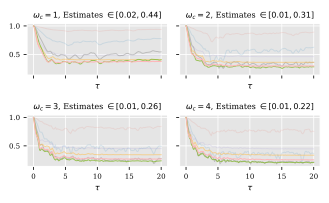
\includegraphics{figs/one_bath_syst/norm_estimate_omega}
  \caption{\label{fig:normest_ω} The maximum norm (for each time
    point) of the first hierarchy states for \(500\) trajectories
    subtracted from norm estimate and normalized by the norm estimate
    for a qubit coupled to single zero temperature ohmic baths
    \cref{eq:one_qubit_model} with varying \(ω_c\). The titles include
    the range of the norm estimates. For higher cutoff frequencies the
    BCF vanishes faster and the norm of the hierarchy states
    decreases. The opacity of the lines is proportional to their
    corresponding \(\abs{G_μ}\). The bound is tightest for the
    hierarchy states with the largest coupling.}
\end{figure}
\begin{figure}[p]
  \centering
  \plot{norm_est/norm_estimate_delta}
  \caption{\label{fig:normest_δ} The same as \cref{fig:normest_ω}, but
    for varying coupling strengths.}
\end{figure}

\subsection{Truncation Scheme}
\label{sec:truncsch}
The norm of the \(\vb{k}\)th hierarchy state scales like
\({1} / {\sqrt{\max_μk_μ}}\). This fact in itself, however, is not
too meaningful as the magnitude of the coupling to the lower hierarchy
states is
\begin{equation}
  \label{eq:couplingmag}
  M_{\vb{k}} = \norm{L} \norm{ψ^{\vb{k}}} \max_μ \abs{\sqrt{G_μk_μ}},
\end{equation}
which balances out the scaling.

Calculating \(M_{\vb{k}}\) explicitly and demanding it to be small
(compared to some energy scale) nevertheless gives a convergent
truncation scheme below a certain coupling strength.
Some basic experimentation has shown, that the cutoff parameter has to
be tuned and is not universally valid which is in accord with the
findings of~\cite{RichardDiss}.

Similarly to~\cite{Shi2009Feb}, a dynamic truncation scheme could also
be implemented.

\section{Some Mathematical Details}
\label{math_detail}

\subsection{Shifted Spectral Densities}
\label{sec:shift_sp}
To provide resonant baths for optimal energy flow, it is useful to
shift the ohmic spectral density to higher frequencies. A more
elaborate way to create resonances would be to use a filter cavity mode
\cite{Kurizki2021Dec} which is left to future work.

The shifted Ohmic-type spectral density is given by
\begin{equation}
  \label{eq:shifted_ohm}
  J(ω) = η \operatorname{Θ}(ω)  \pqty{ω-ω_{s}}^{s} \eu^{-\frac{ω}{ω_{c}}},
\end{equation}
which leads to an additional phase factor in the BCF
\begin{equation}
  \label{eq:shifted_bcf}
  α(τ) = \frac{η}{π}\qty(\frac{ω_c}{1+\iu ω_c τ})^2 \eu^{-\i ω_{s} τ}.
\end{equation}

The finite temperature correlation function of the thermal process
\(ξ\) \cite{RichardDiss} is given by
\begin{equation}
  \label{eq:shifted_thermal}
  \begin{aligned}
    α_{ξ}(τ) &= \frac{1}{π}∫_{0}^{∞}\bose(βω) J(ω) \eu^{-\iu ωτ} \\
    &= \frac{η\operatorname{Γ}(s+1) \eu^{-ω_{s} (\iu τ + β)}}{π β^{1+s}}
  Φ\pqty{\eu^{-ω_{s}β}, s+1, \frac{1+βω_{c}+\iu
      ω_{c}τ}{βω_{c}}}.
  \end{aligned}
\end{equation}

In \cref{eq:shifted_thermal}
\begin{equation}
  \label{eq:lerch}
  Φ=∑_{k=0}^{∞} \frac{z^{k}}{(k+a)^{s}}
\end{equation}
is the Lerch transcendent. For \(\abs{z} \geq 1\) \cref{eq:lerch} is
analytically continued. For \(z=1 \iff ω_{s}=0\) we obtain the Hurwitz
zeta function \(ζ(s, a)\). An efficient and correct numeric
evaluation is, at the time of writing, only available through the
\emph{Arb} library \cite{Johansson2017arb}.

\subsection{Smoothstep Functions}
\label{sec:smoothstep}
The smooth step functions \(S_{n}(x)\) are smooth sigmoid like
versions of the Heaviside step function that are zero except for
\(x\in (0,1)\) and \(n\) times continuously differentiable, even at
the edges.

The polynomial expressions for the smoothstep functions are
\begin{equation}
  \label{eq:smoothstep}
  {S} _{n}(x)={
    \begin{cases}
      0&{\text{if }}x\leq 0\\

      x^{n+1}∑_{k=0}^{n}{\binom {n+k}{k}}{\binom
      {2n+1}{n-k}}(-x)^{k} &{\text{if }}0 < x < 1\\1

       &{\text{if }}1\leq x\\
    \end{cases}}.
\end{equation}

\subsection{Explicit Expressions for the Bath Energy Flow of the QBM
  Model}
\label{sec:explicit_flow}
Here we detail the rest of the calculations omitted in
\cref{sec:bathflow}.

All quantities in \cref{eq:lambdafold} have exponential expansion so
that we can now define\footnote{Note that this is inconsistent with
  \cref{sec:solution}.}
\begin{equation}
  \label{eq:expansions}
  \begin{aligned}
    α_0&=∑_k U_k\eu^{-Q_k t} & \dot{α}_0&=∑_k P_k\eu^{-L_k t} & α(t)
    &= ∑_nG_n\eu^{-W_n t} \\
    A(t) &= ∑_l A_l\eu^{-C_l t} & B(t) &= ∑_l B_l\eu^{-C_l t}.
  \end{aligned}
\end{equation}

With this we can calculate,
\begin{align}
  \label{eq:lambdaintegrals}
  ∫_r^t\dd{s}B(s-r)\dot{α}_0(t-s)
  &=\sum_{m,k}\underbrace{\frac{B_mP_k}{L_k-C_m}}_{\equiv
    Γ^1_{mk}}\qty[\eu^{-C_m(t-r)}-\eu^{-L_k(t-r)}]=g_1(t-r)\\
  ∫_0^{t-r}\dd{u}B(t-r-u)α(u)
  &=\sum_{n,l}\underbrace{\frac{B_nG_l}{C_n-W_l}}_{\equiv
    Γ^2_{nl}}\qty[\eu^{-W_l(t-r)}-\eu^{-C_n(t-r)}]=g_2(t-r)\\
  ∫_0^{r}\dd{u}B(t-r+u)α^\ast(u)
  &=\sum_{n,l}\underbrace{\frac{B_nG_l^\ast}{C_n+W_l^\ast}}_{\equiv
    Γ^3_{nl}}\qty[\eu^{-C_n(t-r)}-\eu^{-W_l^\ast r-C_n t}]=g_3(t,r)
\end{align}
and
\begin{align}
  \label{eq:finalsummands}
  Λ_1(t)& =
                    \begin{aligned}[t]
          ∑_{m,k,n,l}Γ^1_{mk}Γ^2_{nl}\biggl[\frac{1-\eu^{-(C_m+W_l)t}}{C_m+W_l}
                                 &-
                               \frac{1-\eu^{-(C_m+C_n)t}}{C_m+C_n}
                      \\&-
                                 \frac{1-\eu^{-(L_k+W_l)t}}{L_k+W_l}
                                 +
                      \frac{1-\eu^{-(L_k+C_n)t}}{L_k+C_n}\biggr]
                      \end{aligned}\\
  Λ_2(t)&=
          \begin{aligned}[t]
            ∑_{m,k,n,l}Γ^1_{mk}&Γ^3_{nl}\biggl[\frac{1-\eu^{-(C_m+C_n)t}}{C_m+C_n}
           -\frac{1-\eu^{-(L_k+C_n)t}}{L_k+C_n}
            \\&-\frac{\eu^{-(C_n+W_l^\ast)t}-\eu^{-(C_m+C_n)t}}{C_m-W_l^\ast}
            +\frac{\eu^{-(C_n+W_l^\ast)t}-\eu^{-(L_k+C_n)t}}{L_k-W^\ast_l}\biggr]
          \end{aligned}
\end{align}

Also required for \cref{eq:bathderiv_1} are
\begin{align}
  \label{eq:ABconv}
  ∫_0^t\dd{s}A(s)\dot{α}_0(t-s) &= ∑_{n,m}\underbrace{\frac{A_nP_m}{L_m-C_n}}_{\equiv
                                  Γ^A_{nm}}\qty[\eu^{-C_n t}-\eu^{-L_m t}]\\
  ∫_0^t\dd{s}B(s)\dot{α}_0(t-s) &= ∑_{n,m}Γ^1_{nm}\qty[\eu^{-C_n t}-\eu^{-L_m t}]
\end{align}
and
\begin{multline}
  \label{eq:nonzerotemplim}
  ∫_0^t\dd{s}A(s)\qty(α(s)-α_0(s)) =\\
  ∑_{m,n}\frac{A_nG_m}{C_n+W_m}\qty(1-\eu^{-(C_n+W_m)t}) - ∑_{m,n}\frac{A_nU_m}{C_n+Q_m}\qty(1-\eu^{-(C_n+Q_m)t}).
\end{multline}

\subsection{Quantum Brownian Motion with Reversed Time}
\label{sec:reverse_time}
The solution detailed in \cref{sec:oneosc} is only valid for positive
times. Because we strive to employ the same formalism again for
negative times, we will concern ourselves with the transformed
quantities \(\bar{X}(τ) = X(t(τ)) = X(-τ)\) so that \(τ ≥ 0\). It
follows that \(∂_τ \bar{X}(τ) = \bar{X}'(τ) = -\dot{X}(t(τ))\) so that
\begin{align}
  \bar{q}' &= -Ω \bar{p} \label{eq:qtag}\\
  \bar{p}' &= Ω \bar{q} + ∫_0^τ \Im[α_0(τ-s)] \bar{q}(s)\dd{s} - \bar{W}(τ) \label{eq:ptag}
  \\
  \bar{b}'_λ &= \iu g_λ \frac{q'}{2} + \iu\omega_λ b'_λ.
\end{align}
This leads to an equation for \(\bar{G}(τ)\), namely
\begin{equation}
  \label{eq:eqmotpropbar}
  \bar{G}'(τ) = -A \bar{G}(τ) + \int_0^τ K(τ-s) \bar{G}(s)\dd{s}.
\end{equation}
The solution is obtained from the \(t\geq 0\) case by substituting
\(A\rightarrow -A\) and \(K\rightarrow -K\).
We obtain for \(t\leq 0\)
\begin{equation}
  \label{eq:gfinalbar}
  \bar{G}(τ) = G(-τ) = G(t) = \sum_{l=1}^{N+1}\qty[R_l \mqty(\tilde{z}_l & -Ω \\ -\frac{\tilde{z}_l^2}{Ω} & \tilde{z}_l)\eu^{-\tilde{z}_l \cdot
    t} + \cc]
\end{equation}
and
\begin{equation}
  \label{eq:qpsolneg}
  \mqty(q(t)\\ p(t)) = G(t)\mqty(q(0)\\ p(0)) - \int_t^0 G(t-s)
  \mqty(0\\ W(s))\dd{s}.
\end{equation}


\subsection{Detailed Treatment of the Weights in the Normal Ordering
  of the Interaction}
\label{sec:normal_powers}
Notably,
the \(n\)th moment of \(H_\inter\) will depend on the hierarchy states
up to the depth \(n\). However, the terms involving similar exponents
for \(B^\dag\) and \(B\) will have the largest weights, so that the
hierarchy states of depth \(n/2\) play an important role. Truncating
the hierarchy will not simply lead to all higher orders moments of the
interaction being zero. Instead, the dependence upon the hierarchy
states is nontrivial. The explicit appearance of \(α(0)\) can be
avoided if we choose \(B\) unitless and \(α(0) = 1\).

Minimizing the coefficient \(l! 2^l k! (n-2l-k)!\) will give us the
order of \(B\) and thus the hierarchy depth that will contribute the
most to \cref{{eq:interactionnormal}}.  It suffices to minimize the
logarithm,
\begin{equation}
  \label{eq:logcoeff}
  Λ=\ln(2)l + \ln(Γ(l+1)) + \ln(Γ(k+1)) + \ln(Γ(n-2l -k + 1)).
\end{equation}

We begin by minimizing for \(k\)
\begin{equation}
  \label{eq:mink}
  \pdv{Λ}{k} = ψ(k+1)-ψ(n-2l-k+1) \overset{!}{=}0,
\end{equation}
where \(ψ\) is the Digamma function~\cite[p. 136]{NISTHandbook}.
As the Digamma function is strictly monotonic and thus injective,
\cref{eq:mink} implies \(k+1=n-2l-k+1\) and thus
\(l=n/2-k\). Note that the optimizing \(k\) is also the order of the
\(B\) operator associated with the coefficient.

Using this it remains to minimize
\begin{equation}
  \label{eq:logcoeff_k}
  Λ'=\ln(2)\qty(\frac{n}{2}-k) + \ln(Γ\qty(\frac{n}{2}-k+1)) + 2\ln(Γ(k+1)).
\end{equation}
yielding
\begin{equation}
  \label{eq:minkk}
  \begin{aligned}
    \pdv{Λ'}{k} &= 2ψ(k+1) -\ln(2) - ψ\qty(\qty(\frac{n}{2}-k+1))\\
                &\sim 2 \ln(k+1) - \ln(2) -\ln(\frac{n}{2}-k+1)\\
                &\overset{!}{=}0
  \end{aligned}
\end{equation}
and finally
\begin{equation}
  \label{eq:finalk}
  k_m=\left\lceil\sqrt{5+n}-2\right\rceil\sim\sqrt{n},
\end{equation}
where the ceiling has been chosen to obtain an integer. The error this
introduces is of the order of one.  We find that the ``most
important'' order of \(B\) required to calculate \(H_\inter^n\) scales
with \(\sqrt{n}\).  Note however, that the distribution of weights as
shown in~\cref{fig:kdist} will become broader with larger \(n\) and
that a specific \(k\) can occur multiple times, which will slightly
shift the maximum. A binomial (or Gaussian) distribution centered at
\(k_m\) as shown in \cref{fig:kdist} appears to be a good fit for the
relevant parameter space. Such a distribution has a standard deviation
of \(n^{{1}/{4}}\) for large \(n\). The position tail of the \(k\)
distribution thus scales like \(n^{1/2} + n^{1/4}\). The coupling
strength does only enter as a scale that controls which moment of
\(H_I\) is still relevant, albeit such a discussion should rather be
made for centered and normalized moments as they are
dimensionless. Without an a-priori estimate of \(\ev{H_I}\) and the
norm of the hierarchy states the above discussion has to be taken with
a grain of salt. Such estimates may possibly be obtained from the
estimates of the hierarchy state norms in \cref{sec:normest} and
contain not only the coupling strength, but also the shape of the BCF.

The result to take away is, that the expectation value of \(H_I^n\)
depends strongly on hierarchy states of order \(\sim \sqrt{n}\).

\begin{figure}[h]
  \centering
  \plot{interaction_orders/k_weights}
  \caption{\label{fig:kdist}The unnormalized distribution of the
    coefficients in \cref{eq:interactionnormal} with respect to \(k\)
    for different \(n\). As a particular \(k\) can appear multiple
    times in the sum, only the maximal coefficient for each \(k\) is
    being considered in the lines with the triangle markers. The
    maximum of this distribution is given by \cref{eq:finalk}. The
    lines with the circle markers show the full distribution and the
    lines with the triangle markers show only the normalized
    distribution of the maximum of \(l! 2^l k! (n-2l-k)!\) over \(l\).
    The dotted lines correspond to binomial distributions centered at
    \(k_m\).}
\end{figure}

\subsection{Technical Notes on the Code}
\label{sec:code}
